\documentclass[12pt,a4paper]{scrartcl}
\usepackage[utf8]{inputenc}
\usepackage[english,russian]{babel}
\usepackage{indentfirst}
\usepackage{misccorr}
\usepackage{graphicx}
\usepackage{amsmath}
\usepackage{multirow}
\usepackage{pgfplots}
\usepackage{slashbox}
\usepackage[top=1cm, bottom=1cm, left=1cm, right=1cm]{geometry}
\pgfplotsset{compat=1.9}

\begin{document}
	\graphicspath{{C:/Users/Alex/OneDrive/Изображения/TexImgs}}
	
	\newcommand{\ms}{\mathstrut}
	\newcommand{\msp}{\hspace{0.5cm}}
	\newcommand{\al}{\alpha}
	\newcommand{\dg}{^\circ}
	\newcommand{\qd}[2]{^{\frac{#1}{#2}}}
	\newcommand{\qdm}[2]{^{-\frac{#1}{#2}}}
	\newcommand{\lm}[2]{\underset{#1 \rightarrow #2}{\lim}}
	\newcommand{\sfrac}[2]{\dfrac{\strut #1}{\strut #2}}
	\newcommand{\equal}[1]{\overset{(#1)}{=}}
	\newcommand{\linevdots}{\ \raisebox{-.08\height}{\vdots}\ }
	\newcommand{\linecvdots}{\ \raisebox{-.08\height}{\vdots}\hspace{-0.13cm}\raisebox{.15\height}{\cancel{\phantom{a}}\hspace{0.06cm}}}
	\newcommand{\combox}[1]{\ms \msp \msp \begin{minipage}{0.95\linewidth}
			#1
	\end{minipage}}
	
	\newtheorem{pr}{Задача}
	\newtheorem{ex}{Пример}
	\newtheorem{dfn}{Def}
	\newtheorem{theorem}{Th}
	
	\newenvironment{slv}{\ms \msp \textit{Решение:}}{}
	\newenvironment{proof}{\ms \msp \textit{Доказательство: }}{\hfill $\square$}
	
	\begin{titlepage}
		
		\vspace*{\fill}
		
		\begin{center}
			
\includegraphics[scale=0.8]{MIPT.png}
			\\[0.7cm]\Huge Московский Физико-Технический Институт\\(национальный исследовательский университет)
			\\[2cm]\LARGE Отчет по эксперименту
			\\[0.5cm]\noindent\rule{\textwidth}{1pt}
			\\\Huge\textbf{Исследование взаимной диффузии\\газов}
			\\[-0.5cm]\noindent\rule{\textwidth}{1pt}
		\end{center}
		
		\begin{flushleft}
			\textit{Работа №2.2.1; дата: 21.02.22}\hfill\textit{Семестр: 2}
		\end{flushleft}
		
		\vspace*{\fill}
		
		\begin{flushleft}
			Выполнил: \hspace{\fill} Группа:
			\\Кошелев Александр \hspace{\fill} Б05-105
		\end{flushleft}
	\end{titlepage}
	
	%Страница 2
	
	\begin{flushleft}
		\footnotesize{Исследование взаимной диффузии газов} \hspace{\fill} \footnotesize{2}
		\\[-0.3cm]\noindent\rule{\textwidth}{0.3pt}
	\end{flushleft}
	
	\section{Аннотация}
	
	В данной работе изучается взаимная диффузия газов. Дается определение коэффициента взаимной диффузии и изучается влияние рабочего давления системы на коэффициент взаимной диффузии газов на примере пары воздух-гелий.
	
	\textbf{Схема установки:}
	\begin{center}
		\begin{figure}[h]
			\begin{minipage}{0.5\linewidth}
				\begin{center}
					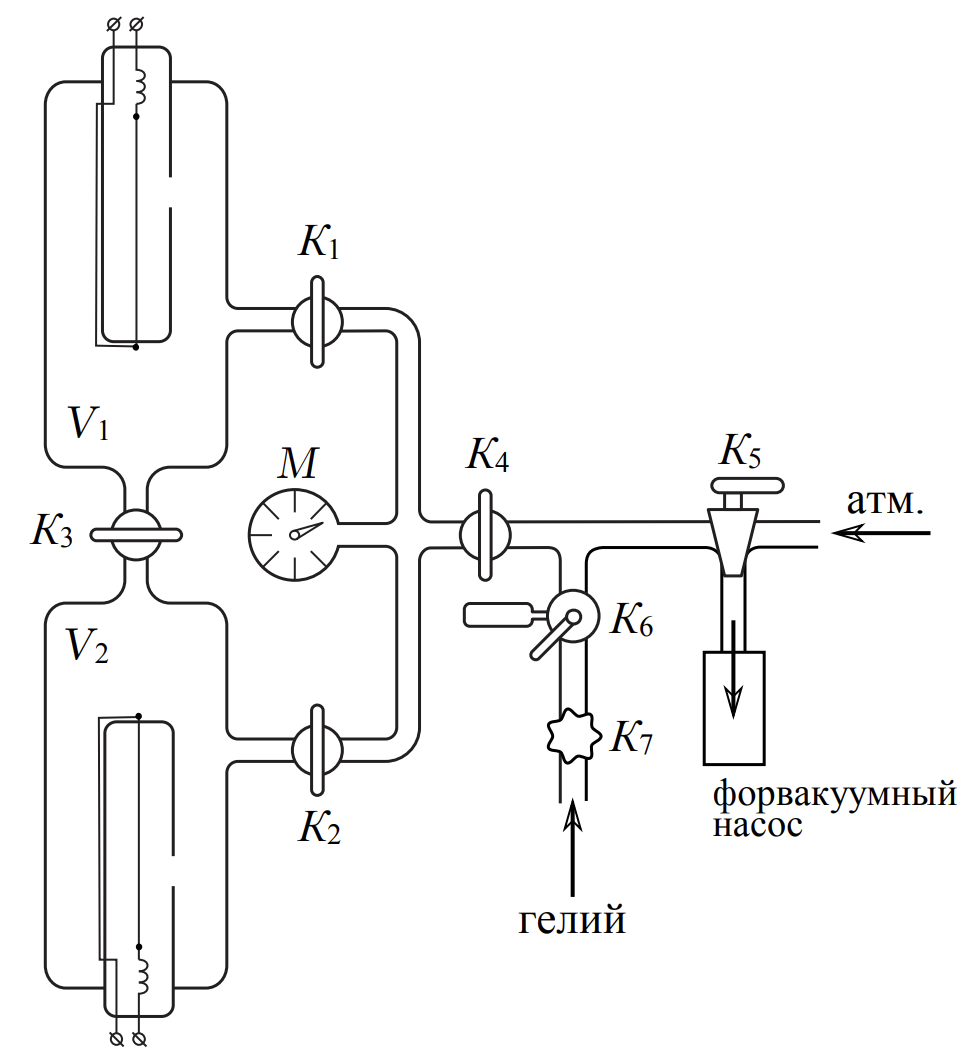
\includegraphics[scale=0.3]{PIC_1.png}
					\\\textbf{Рис. 1:} Схема установки
				\end{center}
			\end{minipage}
		\begin{minipage}{0.5\linewidth}
			\begin{center}
				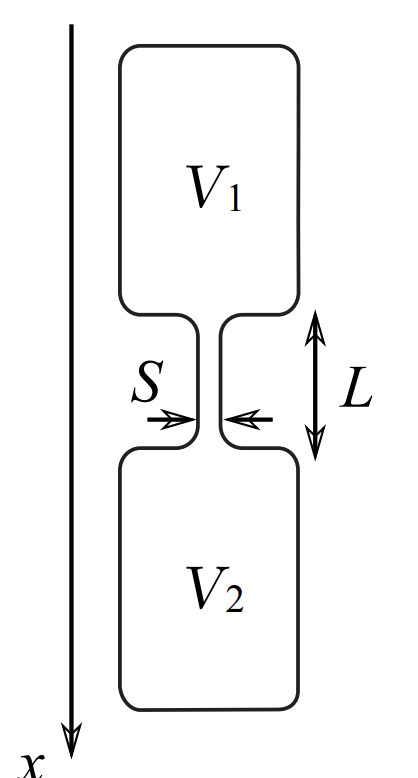
\includegraphics[scale=0.41]{PIC_2.png}
				\\\textbf{Рис. 2:} Схема установки
			\end{center}
		\end{minipage}
		\end{figure}
	\end{center}
	
	\begin{center}
		
	\end{center}
	
	\textbf{В работе используются:} два сосуда для газов $V_1$ и $V_2$, система кранов $K_i$, манометр $M$, баллон сжатого гелия, форвакуумный насос (Рис. 1).
	
	 \medskip
	 Для исследования взаимной диффузии газов и	измерения коэффициента взаимной диффузии $D$ используются два сосуда объёмами $V_1$ и $V_2$ ($V_1 \approx V_2 \equiv V$), соединенные трубкой длины $L$ и сечения $S$ (Рис. 2). Предполагается, что сосуды заполнены смесью двух газов при одинаковом давлении, но с различной концентрацией компонентов. Вследствие взаимной диффузии, проходящей в соединительной трубке, концентрации компонентов в сосудах с течением времени выравниваются. Важно отметить, что диффузия -- относительно медленный процесс, и для его наблюдения необходимо отсутствие конвекции, т. е. макроскопических течений газа. Для этого необходимо обеспечить равенство давлений и температур в сосудах до начала измерений.

	
	\section{Теоретические сведения}
	
	В общем случае концентрации компонентов $n(t, x)$ зависят от как от координаты, так и времени. Задача упрощается, если объём соединительной трубки мал по
	сравнению с объёмами сосудов -- тогда концентрации газов $n_1(t)$ и $n_2(t)$ внутри каждого сосуда можно считать	постоянными по всему объёму сосуда, и принять, что процесс выравнивания концентраций происходит благодаря диффузии в трубке.
	
	Применяя закон Фика в трубке, получим:
	$$j = - D \sfrac{\partial n}{\partial x} = \mathrm{const}$$
	
	%Страница 3
	
	\newpage
	
	\begin{flushleft}
		\footnotesize{Исследование взаимной диффузии газов} \hspace{\fill} \footnotesize{3}
		\\[-0.3cm]\noindent\rule{\textwidth}{0.3pt}
	\end{flushleft}

	Следовательно, распределение концентрации в трубке n(x ) — линейная
	функция:
	$$n(x) = \sfrac{\Delta n}{L}x$$
	
	и плотность потока частиц всюду постоянна и равна
	$$j = -D\sfrac{\Delta n}{L}$$
	
	где $\Delta n = n_2 - n_1$ -- разность концентраций гелия на концах трубки.
	
	Теперь вернёмся к процессу выравнивания концентраций в сосудах.	Частицы перетекают из сосуда 2 в сосуд 1 по трубке и концентрации $n_1(t)$ и $n_2(t)$ меняются во времени. Предположим, что этот процесс происходит достаточно медленно, так что в трубке в любой момент времени успевает установиться практически стационарное течение, описываемое предыдущими формулами. Такое приближение называют квазистационарным. Кроме того, будем считать, что в пределах каждого сосуда частицы распределены равномерно, так что концентрации примеси вблизи трубки и в остальных частях сосуда отличаются мало. Тогда полное число частиц примеси в сосудах равно соответственно $N_1 = n_1V$ и $N_2=n_2V$. Произведение плотности потока $j$ на площадь сечения трубки $S$ даёт количество частиц, пересекающих в единицу времени любое поперечное сечение трубки. Поэтому
	$$\sfrac{\mathrm{d}N_1}{\mathrm{d}t} = jS,\ \sfrac{\mathrm{d}N_2}{\mathrm{d}t} = -jS$$
	
	Выразим отсюда скорость изменения $\Delta n$. Вычитая из второго равенства
	первое и деля результат на объём сосуда $V$, с учетом $j$ получим
	$$\sfrac{\mathrm{d}(\Delta n)}{\mathrm{d}t} = -\sfrac{\Delta n}{\tau}$$
	
	где введено обозначение
	$$\tau = \sfrac{1}{D}\sfrac{VL}{2S}$$
	
	Интегрируя, получаем, что разность концентраций будет убывать по экспоненциальному закону
	$$\Delta n = \Delta n_0 e^{-t/\tau}$$
	
	где $\Delta n_0$ -- разность концентраций примеси в сосудах в начальный момент
	времени. Видно, что величина $\tau$ есть характерное время выравнивания концентраций между сосудами. Оно определяется геометрическими размерами установки и коэффициентом диффузии.
	
	Для измерения разности концентраций в установке применяются датчики теплопроводности. При этом используется	тот факт, что теплопроводность смеси зависит от её состава. При этом для напряжения на парах выполняется:
	$$U = U_0 e^{-t/\tau}$$
	
	%Страница 4
	
	\newpage
	
	\begin{flushleft}
		\footnotesize{Исследование взаимной диффузии газов} \hspace{\fill} \footnotesize{4}
		\\[-0.3cm]\noindent\rule{\textwidth}{0.3pt}
	\end{flushleft}
	
	\section{Проведение эксперимента}
	
	\subsection{Определение вязкости воды}
	
	\paragraph{Измерение параметров установки} \hfill
	
	Занесем в таблицу отношение длины трубки $L/S$ и объем сосудов $V$.
	\begin{center}
		\begin{tabular}{|c|c|}
			\hline
			$L/S$, м$^{-1}$ & $V$, м$^3$ \\\hline
			$1500 \pm 10$ & $(8.00 \pm 0.05) \cdot 10^{-4}$ \\\hline
		\end{tabular}
		\\\textbf{Табл. 1:} Параметры установки 
	\end{center} 

	\paragraph{Измерение коэффициента диффузии} \hfill
	
	Таблицы измерения напряжений очень большие по размеру, поэтому не будем приводить их в данном пункте. Приведем лишь построенный на основании таблицы график и полученные значения $D$ от давления $P$.
	
	\begin{center}
		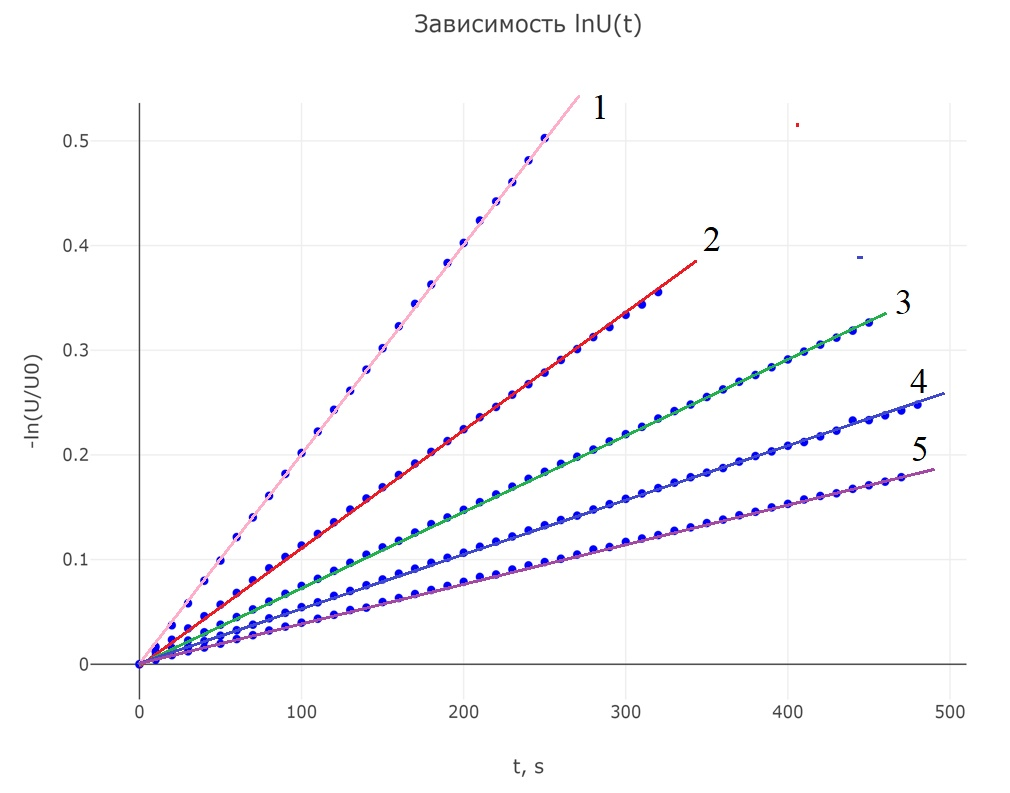
\includegraphics[scale=0.4]{PIC_3.jpg}
		\\\textbf{Рис. 3:} Графики зависимостей $-\ln(U/U_0)(t)$
	\end{center}
	
	Отсюда через коэффициенты наклона получаем

	\begin{center}
		\begin{tabular}{|c|c|c|c|c|c|}
			\hline
			$P$, торр & 40 & 80 & 120 & 180 & 240 \\\hline
			$D \cdot 10^{4}$, м$^2$/с & $12.11 \pm 0.01$ & $6.65 \pm 0.01$ & $4.34 \pm 0.01$ & $3.10 \pm 0.01$ & $2.29 \pm 0.01$\\\hline
		\end{tabular}
		\\\textbf{Табл. 2:} Подсчет коэффициентов диффузии
	\end{center}

	Теперь можно построить зависимость $D(1/p)$, получим вид зависимости и подсчитаем значение в точке, соответствующей атмосферному давлению:
	$$D_0 = (10.9 \pm 1.5) \cdot 10^{-5}\ \text{м}^2/\text{с}$$

	%Страница 5
	
	\newpage
	
	\begin{flushleft}
		\footnotesize{Исследование взаимной диффузии газов} \hspace{\fill} \footnotesize{5}
		\\[-0.3cm]\noindent\rule{\textwidth}{0.3pt}
	\end{flushleft}

	
	\begin{center}
		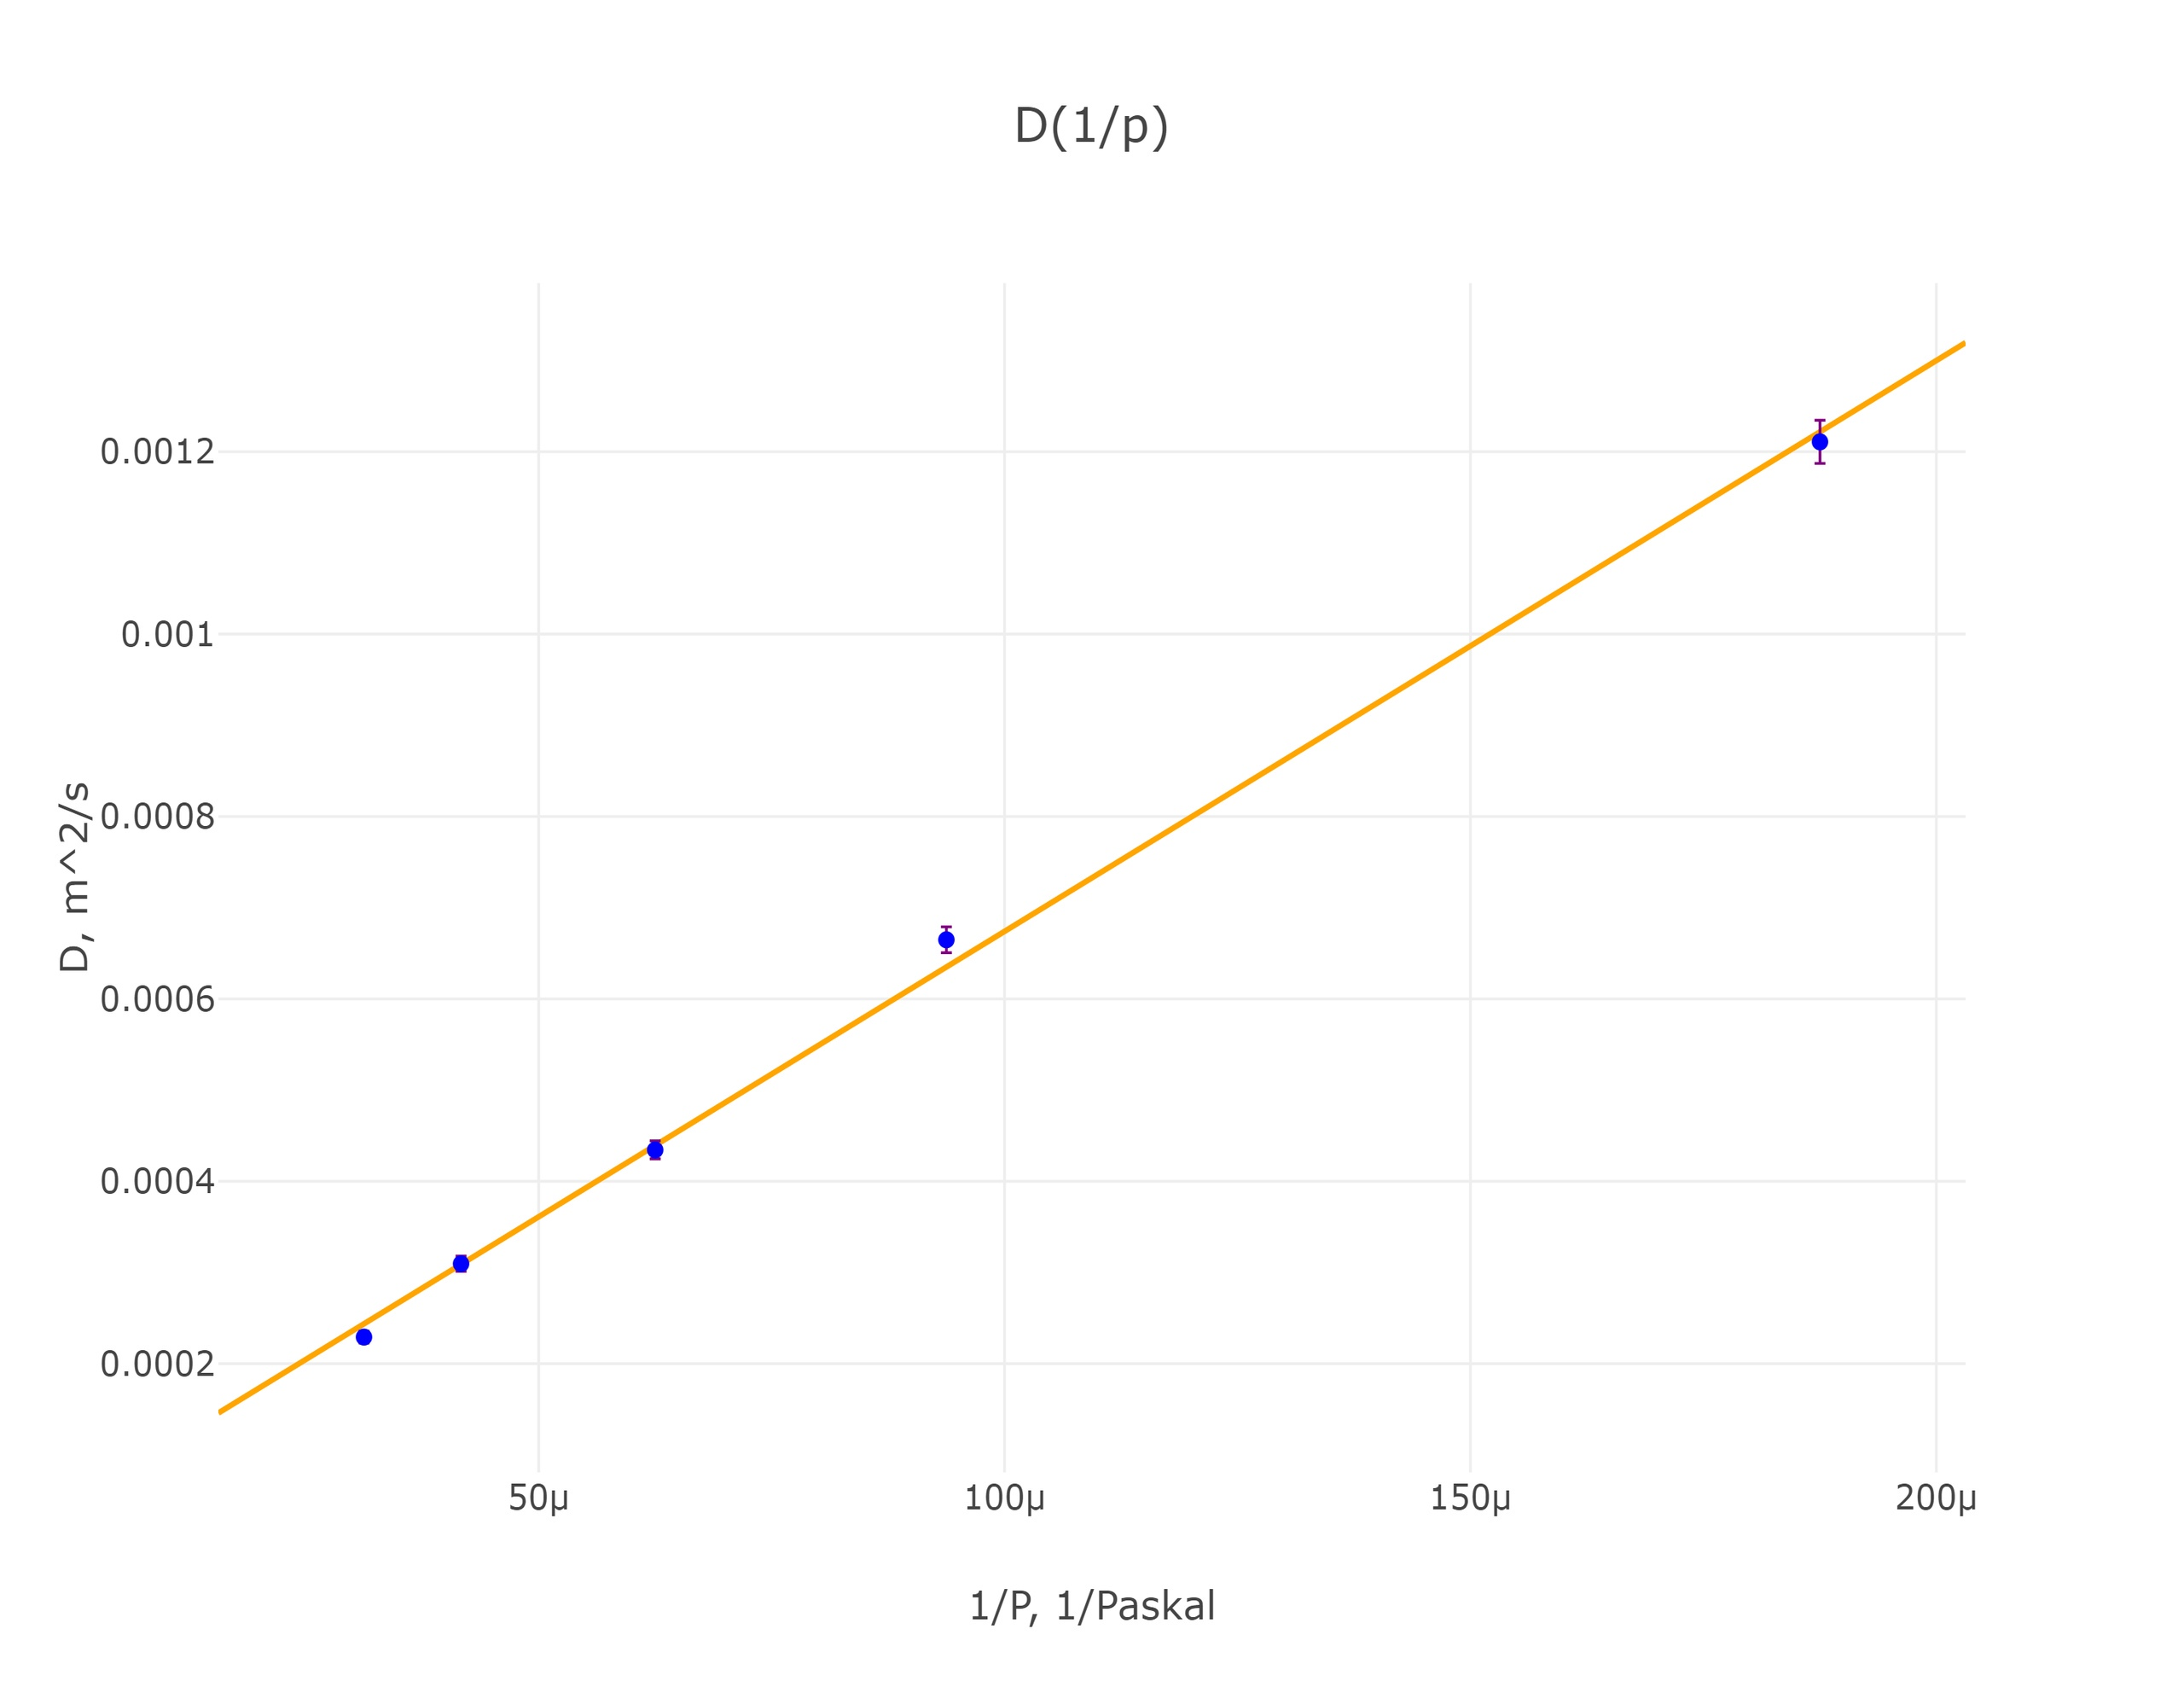
\includegraphics[scale=0.15]{PIC_4.jpg}
		\\\textbf{Рис. 4:} График зависимости $D(1/P)$
	\end{center}
	
	\paragraph{Определение длины свободного пробега и эффективного сечения столкновения атомов гелия с молекулами воздуха}
	
	Из полученных ранее данных определим:
	
	$$\lambda_0 = \sfrac{3D}{\upsilon} = 260 \pm 70\ \text{нм}$$
	
	$$\sigma_0 = \sfrac{kT}{\lambda P} = (1.6 \pm 0.4) \cdot 10^{-19}\ \text{м}^2$$
	
	\section{Выводы}
	
	В ходе работы определено значение коэффициента диффузии пары воздух-гелий при атмосферном давлении $D_0 = (10.9 \pm 1.5) \cdot 10^{-5}\ \text{м}^2/\text{с}$.
	
	Также определена длина свободного пробега $\lambda_0 = 260 \pm 70\ \text{нм}$ и эффективное сечение столкновения стомов гелия с молекулами воздуха.
	
	Все полученные значения совпадают с референсными в пределах 2 величин отклонения.
\end{document}